\documentclass[10pt,twocolumn]{article}
\usepackage[T1]{fontenc}
\usepackage[utf8]{inputenc}
\usepackage{lmodern}
\usepackage[letterpaper,margin=0.75in,columnsep=0.25in]{geometry}
\usepackage{microtype}
\usepackage{amsmath,amssymb}
\usepackage{booktabs,tabularx,array}
\usepackage{graphicx}
\usepackage{tikz}
\usetikzlibrary{arrows.meta,positioning}
\usepackage[numbers,sort&compress]{natbib}
\usepackage{xcolor}
\definecolor{linkblue}{HTML}{174E78}
\usepackage[colorlinks=true,allcolors=linkblue,breaklinks=true]{hyperref}
\usepackage{xurl}
\usepackage{enumitem}
\usepackage{balance}
\setlist{leftmargin=*,nosep}
\setlength{\emergencystretch}{1.5em}
\setlength{\tabcolsep}{4pt}
\newcolumntype{Y}{>{\raggedright\arraybackslash}X}
\newcolumntype{P}[1]{>{\raggedright\arraybackslash}p{#1}}
\newcommand{\vzd}{ViZDoom}
\newcommand{\pending}{\textemdash}
\raggedbottom
\newcommand{\snapshot}{15 September 2026}
\title{ViZDoom Beyond Pixels:\\A Testbed for Multimodal and Generalist Agents}
\author{Research manuscript draft}
\date{\snapshot}
\begin{document}
\maketitle
\begin{abstract}
Evaluating generalist agents requires environments in which perception, memory, and planning have consequences over sustained interaction. ViZDoom provides a first-person setting that connects controlled behavioral tasks with the richer objectives of complete Doom levels. We present its evolution since the previous competition paper, emphasizing audio observations, textual event feedback, semantic object categories, full-level evaluation, and multi-agent interaction through PettingZoo. We also introduce a Model Context Protocol (MCP) server that connects language-model agents to the environment through observation, action, and explicit visual-memory tools. This interface supports the study of both frontier models and the agent harnesses that organize their interaction. We develop an evaluation spanning standard ViZDoom scenarios and the opening levels of Doom and Doom~II, with separate comparisons of model capability, harness design, and sensory information. The resulting research agenda targets multimodal grounding, sparse-reward exploration, and the composition of skills over extended horizons. This draft specifies the methodology and reserves the results presentation; empirical evaluation remains future work.
\end{abstract}
\section{Introduction}
Recognizing a scene and acting successfully within it place different demands on an intelligent system. An agent may correctly identify a door yet fail to return to it after finding a key, or describe an enemy while choosing actions that exhaust its ammunition. Interactive evaluation makes these gaps observable: decisions change the world, errors accumulate, and useful information may disappear before it becomes relevant. Such settings are increasingly important for understanding whether pretrained models can organize perception and tool use into sustained, goal-directed behavior.

\vzd{} offers a compact setting for this question. Agents experience Doom from a first-person perspective and must act under partial observability. Short scenarios isolate behaviors such as aiming, dodging, or navigation. Complete levels combine those behaviors with exploration, resource management, and interactions whose consequences can unfold much later. The shared game mechanics make it possible to examine both individual skills and their composition without changing the underlying world.

This paper revisits \vzd{} since the competition paper first published as a preprint in 2018. Its subsequent development broadens the information agents can receive and the forms of interaction researchers can study. Audio provides evidence about events outside the current view; textual notifications expose concise event feedback; and semantic categories associate visual objects with meaningful roles. Full-level environments make extended objectives easier to study through a common interface, while PettingZoo integration connects multiplayer Doom to the wider multi-agent learning ecosystem.

A further contribution is an MCP server for evaluating language-model agents. It exposes the environment through tools for observation, action, and explicit visual memory, allowing compatible agent systems to engage with the same tasks. This creates two distinct objects of study: the model that interprets observations and chooses actions, and the \emph{harness} that manages its prompts, history, memory, and tool interactions. A capable model may still perform poorly with an unsuitable interaction strategy; conversely, a strong harness may compensate for limitations in individual decisions.

We make four contributions:
\begin{enumerate}[itemsep=3pt]
\item \textbf{Multimodal and semantic observations.} We characterize how audio, text notifications, and object categories extend the questions that can be investigated in a first-person control environment.
\item \textbf{Extended and social interaction.} We position full Doom levels and the PettingZoo wrapper as complementary settings for studying sparse rewards, skill composition, and interaction with other agents.
\item \textbf{An MCP interface for language-model evaluation.} We introduce a server that provides observation, action, and selective visual-memory tools, supporting comparisons of frontier models and their harnesses.
\item \textbf{A research evaluation framework.} We define a study spanning standard \vzd{} scenarios and the opening levels of Doom and Doom~II, with planned measurements of task performance, interaction cost, and failure modes.
\end{enumerate}

Our aim is to connect the library's new capabilities to testable research questions. The manuscript presents the benchmark design and the structure of its empirical evaluation; it does not yet report experimental measurements.

\section{Related Work}
\label{sec:research}
\paragraph{ViZDoom as a research platform.}
\citet{kempka2016vizdoom} introduced \vzd{} as a platform for visual reinforcement learning, enabling controlled first-person tasks and access to game-derived observations. \citet{wydmuch2019competitions} subsequently analyzed agents and evaluation in multiplayer competitions. We use this latter work as the historical reference: its preprint appeared in 2018, followed by the journal publication in 2019. Depth observations, instance labels, map access, and native multiplayer were already part of the platform's earlier scope. The present contribution extends that scope through additional modalities, semantic information, standardized task interfaces, and language-model interaction.

\paragraph{Prediction, control, and memory.}
Several influential studies used \vzd{} to connect perception to decisions over time. In \emph{Learning to Act by Predicting the Future}, \citet{dosovitskiy2017future} selected actions using predicted future measurements, enabling control conditioned on different goals. \citet{lample2017fps} combined recurrent decision-making with auxiliary game-feature prediction for first-person combat. These works established Doom as a setting in which temporally informed representations can support control beyond individual image recognition.

\paragraph{Exploration and world models.}
\citet{pathak2017curiosity} evaluated curiosity-driven exploration in \vzd{}, using prediction error to encourage behavior when external rewards provide little guidance. \citet{savinov2019episodic} investigated episodic curiosity based on reachability and memory, including Doom navigation experiments. \citet{ha2018worldmodels} used the Take Cover scenario to study a controller trained through learned latent dynamics. Together, these studies motivate evaluating exploration, remembered experience, and predictive representations under longer and more varied task dependencies.

\paragraph{Generalization, continual learning, and safety.}
MazeExplorer introduced procedurally generated \vzd{} mazes with separate training and test environments~\citep{harries2019mazeexplorer}. LevDoom studied generalization across levels of environmental difficulty~\citep{tomilin2022levdoom}, while COOM used varied Doom domains and objectives to examine continual reinforcement learning~\citep{tomilin2023coom}. HASARD extended this line of work to vision-based safe reinforcement learning with explicit task rewards and costs~\citep{tomilin2025hasard}. These publications illustrate the value of adapting a shared engine to distinct research questions, and the need to evaluate more than performance on a single familiar scenario.

\paragraph{Learning systems and multi-agent interfaces.}
Sample Factory demonstrated efficient learning and multiplayer self-play in Doom~\citep{petrenko2020samplefactory}, showing how learning infrastructure and agent populations contribute to effective visual control. PettingZoo provides shared interfaces for multi-agent environments~\citep{terry2021pettingzoo}. Integrating \vzd{} with this ecosystem makes its multiplayer tasks more accessible to established multi-agent methods while retaining the game's partially observable interaction setting.

\paragraph{Contemporary agent evaluation.}
Broader research provides context for the proposed benchmark. DreamerV3 demonstrates world-model learning across diverse control domains~\citep{hafner2025dreamer}; BALROG studies language and vision-language models through interactive games~\citep{paglieri2025balrog}; and SIMA~2 investigates generalist agents in virtual worlds~\citep{sima2025}. We cite these as methodological context, rather than as additional examples of \vzd{} use. Procgen emphasizes evaluation over environment distributions~\citep{cobbe2020procgen}, and \citet{agarwal2021precipice} motivate reporting uncertainty and robust aggregate performance instead of relying on isolated point estimates.

MCP supplies a shared protocol through which AI applications access tools and external context~\citep{mcprotocol}. Harbor provides infrastructure for evaluating models and agent systems in containerized tasks~\citep{harborframework}. Our contribution is the \vzd{} interaction server and the associated task and evaluation design. By combining controlled scenarios, full-level objectives, and a common tool interface, the benchmark can examine where failures arise from individual skills, their composition, or the harness that coordinates them.

\section{Extending ViZDoom's Research Scope}
\label{sec:updates}
The additions since the historical platform broaden both the evidence available to an agent and the structure of the tasks it can attempt. Table~\ref{tab:updates} connects each addition to a research question. We distinguish new access to information from inherited engine capabilities: object labels, full-map loading, and multiplayer predate this update, while semantic categories and the newer evaluation interfaces extend their usefulness.

\begin{table*}[t]
\caption{Extensions to \vzd{} and the research questions they enable. The MCP server is the interface for the proposed language-model benchmark; the PettingZoo wrapper is a separate multi-agent integration under development.}
\label{tab:updates}
\small
\begin{tabularx}{\textwidth}{@{}P{0.17\textwidth}P{0.34\textwidth}Y@{}}
\toprule
Extension & Added capability & Research question \\
\midrule
Audio buffer & Access to game sounds alongside the visual stream & When does hearing improve decisions under partial observability? \\
Text buffer & Machine-readable feedback about in-game events & Can agents ground event messages in their actions and remembered state? \\
Label categories & Semantic roles associated with visible objects & Can semantic supervision improve perception and transfer? \\
Full-level environments & A common route to complete Doom-level objectives & Can agents compose local skills into sustained, sparse-reward behavior? \\
PettingZoo wrapper & Standardized interaction with multiple agents & How well do learned strategies transfer across opponents and roles? \\
MCP server & Observation, action, and selective visual-memory tools & How do model capability and harness design affect closed-loop performance? \\
\bottomrule
\end{tabularx}
\end{table*}

\subsection{Audio and Text for Action}
The audio buffer supplements the visual observation with sounds generated by the game. An agent may hear an event that occurs outside its current view or use a sound to distinguish states that look similar. This makes audiovisual control a natural way to study partial observability: the relevant question is whether an additional modality changes a decision, rather than whether a model can recognize the sound in isolation. The standard Basic Audio task provides a controlled example involving an invisible, sound-emitting target.

The text buffer supplies recent in-game notifications. These messages can communicate the outcome of an interaction or a scripted event without requiring the agent to read text from an image. Basic Notifications, for example, uses text to identify which target should be attacked. Such tasks connect language understanding to consequential action while retaining a visually grounded control problem.

Textual feedback is event information, not a general narration of the world. Its usefulness depends on what the scenario communicates, whether that information is already visible, and whether the agent retains it until needed. Comparisons should therefore distinguish the effect of additional information from the effect of presenting the same information in a more accessible form. Audio removal, delayed messages, and matched visual cues provide interventions for studying these differences.

\subsection{Semantic Representations}
Semantic categories extend existing object labels with broader roles, such as enemies, weapons, and players. They support questions about whether agents can learn representations that transfer across changes in appearance while preserving an object's functional role. Category supervision can also connect visual learning to the distinctions that matter for control: avoiding a threat, collecting a resource, or identifying another player.

Two uses deserve separate evaluation. Categories may supervise a perception model during training, with only images supplied at test time; alternatively, category information may be given directly to the acting agent. The latter measures performance with privileged perception and changes the task. Categories are therefore useful both as learning targets and as a diagnostic intervention, but gains in these settings have different interpretations. Custom objects may also require checking that the assigned categories match the intended semantics.

\subsection{Composing Skills in Complete Levels}
Full-level environments provide a common interface to objectives extending beyond the compact scenarios traditionally used in \vzd{}. Doom and Doom~II levels combine navigation and combat with exploration, resource management, and interactions with doors, switches, and keys. The addition is a more accessible route to these tasks; compatibility with Doom maps itself is an inherited capability. Independently reset levels also remain distinct from campaigns that carry inventory and other state across maps.

A terminal completion reward exposes the difficulty of discovering and executing useful intermediate behaviors without dense external guidance. A sequence such as finding a key, remembering a locked door, returning to it, and reaching the exit illustrates the interaction between exploration, memory, and delayed credit. Not every level requires this sequence. The opening maps offer recognizable reference tasks, while stronger claims about long-horizon composition require levels with verified dependencies and backtracking.

Full-level evaluation can thus connect success on isolated scenarios to success on composed objectives. A model that aims reliably but fails to complete a level may have difficulty deciding where to go, managing resources, or recovering from an incorrect plan. These distinctions are more informative than interpreting every failure as a deficit in low-level control.

\subsection{Interaction with Other Agents}
The PettingZoo wrapper connects native multiplayer Doom to a standard multi-agent interface. It supports research on self-play, opponent adaptation, and role-dependent behavior in a shared first-person world. The integration is being developed separately from the main library; its current observation interface is visual, so multimodal support in the core should not be assumed to extend automatically to multiplayer evaluation.

Multi-agent tasks add a source of uncertainty that single-player levels do not capture: other policies change their behavior in response to the agent. Evaluating against held-out opponents and exchanging player roles can reveal whether a strategy is robust or depends on a narrow training interaction. This complements the full-level study, where uncertainty primarily comes from incomplete information about the environment.

\section{An MCP Interface for Agent Evaluation}
\label{sec:mcp}
The MCP server makes \vzd{} available through a common set of tools. An agent can inspect the current state, execute an action, save a visual state under an identifier, and retrieve a previously saved state. These operations connect a model's decisions to a persistent environment and provide explicit support for selective memory. Figure~\ref{fig:interaction} summarizes the interaction.

\begin{figure}[t]
\centering
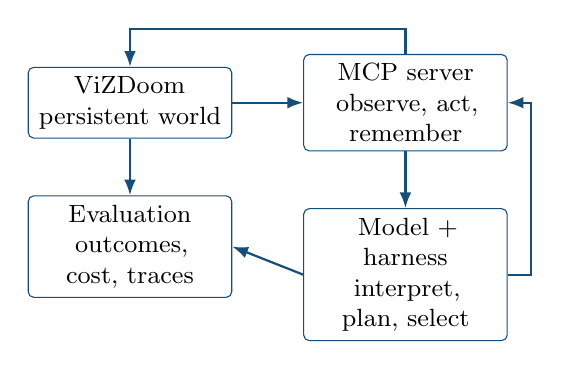
\begin{tikzpicture}[
 box/.style={draw=linkblue,rounded corners=2pt,align=center,font=\small,minimum height=0.68cm,text width=2.35cm},
 flow/.style={-{Latex[length=2mm]},draw=linkblue,thick}]
\node[box] (world) {ViZDoom\\persistent world};
\node[box,right=0.9cm of world] (tools) {MCP server\\observe, act, remember};
\node[box,below=0.72cm of tools] (agent) {Model + harness\\interpret, plan, select};
\node[box,below=0.72cm of world] (eval) {Evaluation\\outcomes, cost, traces};
\draw[flow] (world.east) -- (tools.west);
\draw[flow] (tools.south) -- (agent.north);
\draw[flow] (agent.east) -- ++(0.3,0) |- (tools.east);
\draw[flow] (tools.north) -- ++(0,0.32) -| (world.north);
\draw[flow] (world.south) -- (eval.north);
\draw[flow] (agent.west) -- (eval.east);
\end{tikzpicture}
\caption{Closed-loop interaction through MCP. The harness organizes model calls, history, and memory; the server mediates access to the game. Evaluation uses environment outcomes and interaction records.}
\label{fig:interaction}
\end{figure}

\subsection{Observation and Action}
The server presents the current first-person image together with task and episode information. Actions select game controls and their duration, after which the agent receives an updated observation. Synchronous interaction lets the model deliberate between actions without the world advancing during inference; action duration still determines how much game activity occurs before the next observation.

The existing full-level tasks also provide an automap. This is meaningful assistance for navigation and will be retained in the reference condition and removed in a separate ablation. Episode feedback can include game variables and rewards, so the reference condition should be understood as a tool-mediated observation setting with declared assistance. A stricter visual condition must control those channels explicitly. The current MCP interface supplies images and structured feedback; exposing the core audio and notification buffers through it is a planned extension, not an established property of this interface.

\subsection{Selective Visual Memory}
The memory tools allow an agent to save a state it considers useful and retrieve it later. Possible uses include remembering a junction, a previously closed door, or a location associated with a task-relevant event. Retrieval is limited to explicitly stored states, making the decision to remember part of the agent's behavior.

This mechanism supports experiments on memory selection and use. Does an agent save observations that later matter? Does retrieval change an ineffective action sequence? Does a bounded collection of visual memories help more than a textual summary of the same interaction? These questions require controlling the harness's ordinary conversation history, since retaining every previous image would provide a second memory mechanism. Performance alone should be complemented by analyses of what was stored, what was retrieved, and what the agent subsequently did.

\subsection{Separating Models and Harnesses}
The benchmark distinguishes three comparisons. A \emph{model comparison} places different models behind the same harness, with matched instructions, tool access, and interaction limits. A \emph{harness comparison} holds the model fixed while varying history management, explicit memory, or planning. A \emph{system comparison} evaluates a supported model together with its native agent harness.

The existing evaluation integration supports Codex and Claude Code through Harbor, alongside the possibility of a common evaluation harness. These provide meaningful complete-system comparisons, but differences between native systems cannot automatically be attributed to the model or to the harness alone. A crossed comparison should be made only where the same model can actually be used through both interfaces. Frontier model identities will be selected and recorded when the evaluation is frozen, rather than inferred from example defaults.

The server also records interactions for later analysis. Task success must be established from environment events, rather than from the agent's claim that it has finished. Any brief decision notes produced by the agent are self-reports of its intended behavior; they are not direct evidence of internal reasoning. Outcome records, actions, and retrieved observations together provide a basis for examining failures without relying on those self-reports alone.

\section{Experimental Design}
\label{sec:experiments}
The proposed evaluation asks four questions: (1) how well frontier models perform on individual \vzd{} skills; (2) how much harness design affects their performance; (3) whether those skills compose into full-level completion; and (4) when additional sensory information or memory changes the outcome. The first study centers on language-model agents. Multimodal learning and multi-agent experiments provide complementary follow-up studies.

\subsection{Task Suite}
\paragraph{Standard scenarios.}
The standard suite spans target selection and aiming, navigation, combat, and survival. Basic, Predict Position, and My Way Home isolate relatively compact objectives. Deadly Corridor combines progress toward a goal with threats along the route. Defend the Center, Defend the Line, and Deathmatch emphasize combat and resource use; Health Gathering, Health Gathering Supreme, and Take Cover emphasize survival. Basic Audio and Basic Notifications introduce controlled sensory requirements. Table~\ref{tab:standard-results} reserves results for all twelve environments. The current MCP task set includes Basic and My Way Home; the remaining standard scenarios require task-specific integration and outcome validation before evaluation.

\paragraph{Opening Doom levels.}
The primary full-level comparison uses \emph{Hangar}, the first level of Doom, and \emph{Entryway}, the first level of Doom~II. Both are already represented in the MCP task set. The second levels, \emph{Nuclear Plant} and \emph{Underhalls}, form an extended opening-level comparison and are also represented in that set. We evaluate each level from an independent starting state, with completion defined by reaching a valid exit.

These familiar levels provide interpretable reference tasks, not a test of unseen-map generalization. They also differ in the interactions needed to reach an exit. Before evaluation, we will annotate required keys, switches, and backtracking so that success is interpreted in relation to the actual dependencies of each map. A later transfer study will use held-out authored or generated layouts, with redistributable content where possible, to distinguish familiarity from general control capability.

\subsection{Comparison Conditions}
We plan to evaluate at least three frontier vision-language models using a common harness. Model selection will reflect availability at the evaluation freeze and include multiple model families. Compatible native systems using Codex and Claude Code will be evaluated separately. All systems will receive the same task objectives, game controls, and observation privileges within a comparison. Model-specific preprocessing and unavailable model--harness combinations will be disclosed.

Within a fixed model, we will compare a common harness with bounded history, the same harness with selective visual memory, and a variant that adds structured planning within the same total budget. Disabling memory must remove both storage tools and any equivalent harness-provided persistent store. Ordinary conversation history will remain matched. An automap ablation on the full levels will isolate the effect of that additional spatial information.

Random-action and reactive heuristic agents will establish task sanity checks. Feed-forward and recurrent reinforcement-learning policies will provide learned baselines under declared training budgets. These policies are reference points for different learning regimes: their task-specific training is not directly comparable to the unknown pretraining resources of frontier models. A matched-control comparison will give all agents the same permitted action durations and observations; any results from a different native RL interface will be presented separately.

\subsection{Evaluation Protocol}
All conditions will use the same prespecified episode seeds and starting rules for each task. The initial plan uses 30 paired episodes per task and inference condition; feasibility pilots may revise this count before the test protocol is frozen. Learned RL baselines will use five independent training seeds, each evaluated on the same episode suite. We will fix inference settings, action limits, and model choices before final evaluation and use separate validation tasks to choose prompts and harness settings.

The primary full-level objective is sparse completion reward:
\begin{equation}
 r_t^{\mathrm{ext}}=\mathbb{1}\{\text{a valid level exit occurs at }t\}.
\end{equation}
No intermediate progress reward will be supplied in this condition. Standard scenarios will retain their declared task objectives and report native return alongside the relevant behavioral outcome. Episode termination, death, and budget exhaustion will be recorded separately; a positive intermediate reward is not a general definition of success.

Budgets will separately constrain simulated game time, model calls, generated tokens, and elapsed wall time. The evaluation will record actual game advancement, since one tool call may contain several repeated actions. Primary comparisons will use a common interaction allowance, followed by performance-versus-cost analyses. Synchronous stepping measures control with deliberation between actions; it does not establish performance under real-time deadlines.

\subsection{Measures and Analysis}
For finite-goal tasks, the main outcome is the probability of completing the objective. Combat scenarios will report return and kills; survival scenarios will report survival duration. Completion times will be reported together with failures, preventing a system that succeeds only on easy episodes from appearing efficient solely through success-conditioned averages. Additional measures include model calls, tokens, billed inference cost, invalid actions, and repeated ineffective actions.

Full-level completion will be reported separately for each map. A summary across the two primary maps will give each map equal weight. The standard finite-goal summary will likewise average success rates over a fixed subset: Basic, My Way Home, Deadly Corridor, and Predict Position. Audio- and text-dependent tasks will be reported separately until all compared systems receive the required modality. Native returns with different meanings and scales will not be averaged into a single score.

We will report 95\% confidence intervals and paired differences between prespecified conditions. For trained policies, resampling will respect independent training runs rather than treating all evaluation episodes as independent agents. Uncertainty on the four opening maps will be conditional on that fixed suite; it cannot support a claim about an arbitrary population of Doom levels. Failures in infrastructure and interrupted episodes will be accounted for explicitly, with rerun rules fixed before evaluation.

Interaction traces will support a failure taxonomy covering perceptual errors, ineffective control, missed interactions, loss of spatial context, resource depletion, and failure to revise a plan. Coding rules will be defined before the final trace review, with independent annotation of a subset to assess agreement. Agent-written explanations may aid inspection but will not determine the assigned cause without behavioral evidence.

\subsection{Follow-up Studies}
Modality studies will compare vision with audiovisual and visual-plus-notification conditions on tasks where those channels provide identifiable evidence. Corrupted or removed cues will test whether an agent actually uses the information. Semantic categories will be evaluated separately as training-only supervision and as privileged test-time input. Native audio and text must first be exposed through the MCP interface for corresponding language-model comparisons.

The multi-agent study will compare fixed-opponent training, self-play, and population-based training through the PettingZoo wrapper. Evaluation will use held-out opponents, exchanged player roles, and cross-play outcomes on unseen maps. These studies extend the benchmark's research scope, while the initial empirical priority remains standard-scenario and opening-level performance of frontier models and harnesses.

\section{Results: Planned Presentation}
\label{sec:results}
This section reserves the empirical presentation for the planned evaluation. \textbf{No measurements have been collected for this manuscript.} An em dash denotes a pending measurement, not zero performance or an unavailable system. Labels C1--C3 denote frontier-model slots in the common harness; N1--N2 denote supported native systems. The final model names will replace these labels at the evaluation freeze. Unsupported model--harness or modality combinations will be marked explicitly rather than assigned a score.

\subsection{Frontier Models and Agent Systems}
Table~\ref{tab:model-results} will summarize task completion and inference cost. Common-harness rows will support comparisons among models; native-system rows will characterize the deployed model--harness combination. The analysis will report uncertainty and per-task variation before discussing any ranking. It will examine whether success on compact objectives predicts success on complete levels and whether differences persist at comparable interaction cost.

\begin{table*}[t]
\caption{Reserved comparison of frontier models and native agent systems. Goal SR is the macro-average success rate on the four standard finite-goal tasks defined in Section~\ref{sec:experiments}. Hangar and Entryway are the primary full-level tasks. Cost is mean billed inference cost per episode over those same six tasks, with tasks weighted equally. All scores and costs are pending; the completed table will include 95\% confidence intervals for success rates.}
\label{tab:model-results}
\small
\begin{tabularx}{\textwidth}{@{}l Y l c c c c@{}}
\toprule
ID & Model slot & Harness & Goal SR (\%) & Hangar (\%) & Entryway (\%) & Cost (USD) \\
\midrule
C1 & Frontier model 1 & Common & \pending & \pending & \pending & \pending \\
C2 & Frontier model 2 & Common & \pending & \pending & \pending & \pending \\
C3 & Frontier model 3 & Common & \pending & \pending & \pending & \pending \\
N1 & Compatible model & Codex & \pending & \pending & \pending & \pending \\
N2 & Compatible model & Claude Code & \pending & \pending & \pending & \pending \\
\bottomrule
\end{tabularx}
\end{table*}

\subsection{Standard ViZDoom Environments}
Table~\ref{tab:standard-results} reserves a task-level profile across the standard environments. It will distinguish navigation and finite-goal control from combat and survival. Return, kill counts, and survival duration will accompany the primary measures where relevant. The sensory tasks will additionally compare intact and ablated observations. Performance differences will be interpreted within each task's objective rather than through an average of unrelated reward scales.

\begin{table*}[t]
\caption{Reserved results on the standard \vzd{} environments. FF-RL and RNN-RL denote planned feed-forward and recurrent learned baselines; C1--C3 use the common harness. SR means objective success rate. Survival is measured in simulated seconds. Every measurement is pending. $\dagger$ marks tasks requiring audio or notification support in the MCP interface before the relevant language-model evaluation. Native-system profiles will use the same task breakdown.}
\label{tab:standard-results}
\small
\begin{tabularx}{\textwidth}{@{}Y P{0.24\textwidth}ccccc@{}}
\toprule
Environment & Primary measure & FF-RL & RNN-RL & C1 & C2 & C3 \\
\midrule
Basic & Target elimination SR (\%) & \pending & \pending & \pending & \pending & \pending \\
Basic Audio$^\dagger$ & Target elimination SR (\%) & \pending & \pending & \pending & \pending & \pending \\
Basic Notifications$^\dagger$ & Correct-target SR (\%) & \pending & \pending & \pending & \pending & \pending \\
Deadly Corridor & Goal SR (\%) & \pending & \pending & \pending & \pending & \pending \\
Deathmatch & Episode return & \pending & \pending & \pending & \pending & \pending \\
Defend the Center & Episode return & \pending & \pending & \pending & \pending & \pending \\
Defend the Line & Episode return & \pending & \pending & \pending & \pending & \pending \\
Health Gathering & Survival (s) & \pending & \pending & \pending & \pending & \pending \\
Health Gathering Supreme & Survival (s) & \pending & \pending & \pending & \pending & \pending \\
My Way Home & Goal SR (\%) & \pending & \pending & \pending & \pending & \pending \\
Predict Position & Target elimination SR (\%) & \pending & \pending & \pending & \pending & \pending \\
Take Cover & Survival (s) & \pending & \pending & \pending & \pending & \pending \\
\bottomrule
\end{tabularx}
\end{table*}

\subsection{Opening Doom Levels}
Table~\ref{tab:level-results} reserves completion rates for the two primary levels and the extended pair. For each level, the final presentation will include completion-time distributions, deaths, budget exhaustion, and the most common observed failure categories. A companion analysis will compare the reference automap condition with first-person observations alone. These results will test composition on the named levels; transfer to unfamiliar maps will remain a separate claim.

\begin{table*}[t]
\caption{Reserved level-completion success rates (\%) for the opening levels of Doom and Doom~II. Hangar and Entryway form the primary comparison; Nuclear Plant and Underhalls extend it to the second level of each game. C1--C3 and N1--N2 are defined in Table~\ref{tab:model-results}. All entries are pending and will be reported with 95\% confidence intervals.}
\label{tab:level-results}
\small
\begin{tabularx}{\textwidth}{@{}l Y l ccccc@{}}
\toprule
Game & Level & Role & C1 & C2 & C3 & N1 & N2 \\
\midrule
Doom & Hangar (E1M1) & Primary & \pending & \pending & \pending & \pending & \pending \\
Doom II & Entryway (MAP01) & Primary & \pending & \pending & \pending & \pending & \pending \\
Doom & Nuclear Plant (E1M2) & Extended & \pending & \pending & \pending & \pending & \pending \\
Doom II & Underhalls (MAP02) & Extended & \pending & \pending & \pending & \pending & \pending \\
\bottomrule
\end{tabularx}
\end{table*}

\subsection{Harness and Memory Ablations}
Table~\ref{tab:harness-results} reserves a within-model comparison of memory and planning. We will relate completion to the number of model calls and the use of stored observations, and examine whether retrieval precedes useful behavioral changes. Additional cost curves will show the trade-off between interaction resources and completion. A native-harness comparison using the same model will be added only when that pairing is supported; otherwise it belongs to the complete-system comparison.

\begin{table*}[t]
\caption{Reserved harness ablation, holding the model, observation privileges, base history policy, and total budgets fixed. Calls and retrievals are per-episode means over the six primary tasks used in Table~\ref{tab:model-results}, with tasks weighted equally. A dash denotes a pending observation; ``disabled'' is an experimental condition. The model will be named when selected.}
\label{tab:harness-results}
\small
\begin{tabularx}{\textwidth}{@{}Y ccccc@{}}
\toprule
Harness condition & Goal SR (\%) & Hangar (\%) & Entryway (\%) & Model calls & Retrievals \\
\midrule
Common, bounded history & \pending & \pending & \pending & \pending & Disabled \\
Common + visual memory & \pending & \pending & \pending & \pending & \pending \\
Common + memory + planning & \pending & \pending & \pending & \pending & \pending \\
\bottomrule
\end{tabularx}
\end{table*}

\section{Discussion and Limitations}
The proposed benchmark treats \vzd{} as a setting for studying components of general agency: integrating observations, acting toward goals, using memory, and composing behavior over time. Completion of a finite collection of Doom tasks would provide evidence about those capabilities in this domain. It would not establish general intelligence or broad transfer outside the game. The empirical evaluation must determine whether the tasks discriminate among current systems and which differences are stable across runs.

Public Doom levels may be familiar from model pretraining, walkthroughs, or previous benchmarks. Their value as interpretable reference tasks should therefore be separated from claims about generalization. Even with unfamiliar layouts, an agent may benefit from prior knowledge of game mechanics. Future evaluation should distinguish this useful prior knowledge from memorized routes, while using independently authored or generated maps to test adaptation.

Observation access also shapes the task. Automaps, game variables, text notifications, and perfect semantic categories can remove uncertainty that would otherwise require perception or memory. Such assistance is a useful experimental intervention when declared and controlled. Comparisons across different observation privileges, action timing, or training regimes cannot be reduced to a single ordering of agent capability.

The breadth of the library exceeds the scope of the initial MCP benchmark. Audio and notification tools still need to be integrated into that interface, and the PettingZoo wrapper remains a separate development effort. Their evaluation should follow the validation of each observation and task contract. More generally, synchronous gameplay favors agents that can deliberate between actions; a later real-time study would test an additional capability under latency constraints.

Finally, a sparse outcome alone rarely explains failure. The combination of task-level measures and interaction traces is intended to make negative results informative, while keeping diagnostic information separate from what the agent receives. The current manuscript provides that evaluation structure. Claims about performance, modality benefits, or the value of a particular harness remain contingent on the planned experiments.

\section{Conclusion}
\vzd{} has evolved from a primarily visual control platform toward a testbed for multimodal, extended, and social interaction. Audio, textual feedback, semantic categories, full-level tasks, and PettingZoo integration broaden its research scope. The MCP server adds a common route for language-model agents to observe, act, and maintain selective visual memories. Together, these developments support an evaluation that connects standard scenario skills with the opening levels of Doom and Doom~II, while distinguishing the effects of models, harnesses, and observation access. The proposed study and reserved results tables provide the basis for assessing that contribution empirically.

\balance
\bibliographystyle{plainnat}
\bibliography{references}
\end{document}
